\newpage

\anonchapter{Лабораторная работа №5}
\setcounter{chapter}{5}

\begin{center}
Исследование магнетосопротивления полупроводников\\
(4 часа)
\end{center}

\section{Цель работы}
Измерение изменения сопротивления полупроводников в магнитном поле, определение дрейфовой подвижности носителей заряда.

\section{Теоретическая часть}

\subsection{Увеличение электросопротивления полупроводника в магнитном поле}

Эффект магнетосопротивления заключается в изменении электросопротивления обазца при наложении магнитного поля. Причиной визникновения этого эфекта является искривление траектории движения носителей заряда в скрещенных магнитном и электрическом полях.

\begin{figure}[h!]\centering
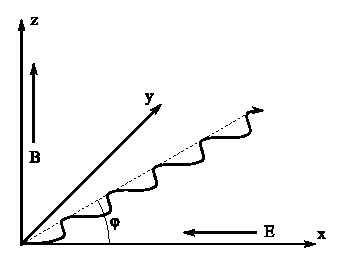
\includegraphics[height=6cm]{pic5_cycloid.eps}
\caption{Траектория электрона в скрещенных электрическом и магнитном полях внутри полупроводника}
\label{pic5_cycloid}
\end{figure}

На движущийся заряд в магнитном поле действует сила Лоренца, которая направлена перпендикулярно дрейфовой скорости электронов $\overrightarrow{V}_{d}$ и вектору магнитной индукции $\overrightarrow{B}$. В полупроводнике заряд не может двигаться сколь угодно долго вдоль идеальной траектории, так как испытывает периодические столкновения с дефектами кристаллической решётки. При столкновении теряется энергия и, следовательно, скорость. Таким образом, носители заряда в кристалле двигаются по отрезкам циклоиды (см. рисунок \ref{pic5_cycloid}), при этом среднее направление их движения составляет с направлением поля $\overrightarrow{E}$ некоторый угол $\phi$, называемый углом Холла. Величина угла Холла определяется соотношением между дрейфовой подвижностью носителей $\mu_{d} $ и индукцией магнитного поля:

\begin{equation}
\tg \phi = \mu_{d} B
\end{equation}

Из-за того, что частица движется не по прямой, за время свободного пробега она проходит вдоль поля расстояние меньшее, чем длина свободного пробега $l_{0}$:

\begin{equation}
l_{\text{х}} = l_{0} \cos \phi
\end{equation}

В слабых магнитных полях при малом значении угла Холла

\begin{equation}
l_{\text{х}} = l_{0} \left( 1-\frac{\phi^2}{2} \right) = l_{0} \left( 1-\frac{\mu_{d}^2 B^2}{2} \right)
\end{equation}

Уменьшение пути $l_{\text{х}}$ эквивалентно уменьшению проводимости проводника:

\begin{equation}
\frac{\Delta \rho}{\rho_{0}} = \frac{\rho_{B} - \rho_{0}}{\rho_{0}} = \frac{\sigma_{0} - \sigma_{B}}{\sigma_{B}} = \frac{\l_{0} - \l_{\text{х}}}{\l_{\text{х}}} \approx \frac{\mu_{d}^2 B^2}{2}
\end{equation}

Изменение электросопротивления полупроводника пропорционально квадрату индукции магнитного поля, при этом коэффициент пропорциональности определяется величиной дрейфовой подвижности.

